% Paquets généraux
\documentclass[a4paper,12pt,titlepage]{article}
\usepackage[T1]{fontenc}
\usepackage[utf8]{inputenc}
\usepackage[french]{babel}
\usepackage[gen]{eurosym}
%\usepackage[dvips]{graphicx}
\usepackage{fancyhdr}
\usepackage{pdfpages} 
\usepackage{multido}
\usepackage{hyperref}
%\usepackage{textcomp}
%\usepackage{aeguill}
\usepackage{schemabloc}
\usepackage[bitstream-charter]{mathdesign}
\usepackage{minted}

\newcommand{\id}{71}
\newcommand{\nom}{Théorie des mécanismes}
\newcommand{\sequence}{04}
\newcommand{\nomsequence}{Liaisons entre les solides}
\newcommand{\num}{02}
\newcommand{\type}{KH}
\newcommand{\descrip}{Liaisons équivalentes, hyperstatisme, liaisons en série et en parallèle, théorie des graphes}
\newcommand{\competences}{B2-12: Proposer une modélisation des liaisons avec leurs caractéristiques géométriques. \\ &  B2-13: Proposer un modèle cinématique paramétré à partir d'un système réel, d'une maquette numérique ou d'u \\ &  B2-17: Simplifier un modèle de mécanisme. \\ &  B2-18: Modifier un modèle pour le rendre isostatique. \\ &  C1-04: Proposer une démarche permettant d'obtenir une loi entrée-sortie géométrique.  \\ &  C2-05: Caractériser le mouvement d'un repère par rapport à un autre repère. \\ &  C2-06: Déterminer les relations entre les grandeurs géométriques ou cinématiques. }
\newcommand{\nbcomp}{7}
\newcommand{\systemes}{}
\newcommand{\systemesnum}{}
\newcommand{\systemessansaccent}{}
\newcommand{\ilot}{2}
\newcommand{\ilotstr}{02}
\newcommand{\dossierilot}{\detokenize{Ilot_02 }}


\newcommand{\auteurun}{Renaud Costadoat}
\newcommand{\auteurdeux}{Françoise Puig}
\newcommand{\institute}{Lycée Dorian}


\usepackage{color}
\usepackage{xcolor}
\usepackage{colortbl}
\usepackage{helvet}
\usepackage[frenchmath]{newtxsf} % for sans serif symbols
\renewcommand{\familydefault}{\sfdefault}
%\usepackage{amsfonts}
%\usepackage{amsmath}
%\usepackage{lmodern}
\usepackage{mathastext}
%\usepackage{xspace}
\usepackage{varioref}
\usepackage{tabularx}
%\usepackage{floatflt}
\usepackage{graphics}
\usepackage{wrapfig}
\usepackage{textcomp}
\usepackage{tikz}
\usepackage{wrapfig}
\usepackage{gensymb}
\usepackage[european]{circuitikz}
\usetikzlibrary{babel}
\usepackage{ifthen}
\usepackage{cancel}
\usepackage{etoolbox}
\usepackage{multirow}
%\usepackage{boxedminipage}
\definecolor{gris25}{gray}{0.75}
\definecolor{bleu}{RGB}{18,33,98}
\definecolor{bleuf}{RGB}{42,94,171}
\definecolor{bleuc}{RGB}{231,239,247}
\definecolor{rougef}{RGB}{185,18,27}
\definecolor{rougec}{RGB}{255,188,204}%255,230,231
\definecolor{vertf}{RGB}{103,126,82}
\definecolor{vertc}{RGB}{220,255,191}
\definecolor{forestgreen}{rgb}{0.13,0.54,0.13}
\definecolor{blcr}{rgb}{0.59,0.69,0.84}
\definecolor{blfr}{rgb}{0.32,0.51,0.75}
\definecolor{orfr}{rgb}{0.90,0.42,0.15}
\definecolor{orcr}{rgb}{0.90,0.65,0.50}
\definecolor{orangef}{rgb}{0.659,0.269,0.072}
\definecolor{orange}{rgb}{0.58,0.35,0.063}
\definecolor{orangec}{rgb}{0.43,0.32,0.25}
\definecolor{rcorrect}{rgb}{0.6,0,0}
\definecolor{sequence}{rgb}{0.75,0.75,0.75}
\definecolor{competences}{rgb}{0.61,0.73,0.35}
\definecolor{grisf}{HTML}{222222}
\definecolor{grisc}{HTML}{636363}
\definecolor{normal}{HTML}{4087c4}
\definecolor{info}{HTML}{5bc0de}
\definecolor{success}{RGB}{92,184,92}
\definecolor{warning}{RGB}{240,173,78}
\definecolor{danger}{RGB}{217,83,79}
\hypersetup{                    % parametrage des hyperliens
    colorlinks=true,                % colorise les liens
    breaklinks=true,                % permet les retours à la ligne pour les liens trop longs
    urlcolor= blfr,                 % couleur des hyperliens
    linkcolor= orange,                % couleur des liens internes aux documents (index, figures, tableaux, equations,...)
    citecolor= forestgreen                % couleur des liens vers les references bibliographiques
    }

% Mise en page
\pagestyle{fancy}

\setlength{\hoffset}{-18pt}

\setlength{\oddsidemargin}{0pt} 	% Marge gauche sur pages impaires
\setlength{\evensidemargin}{0pt} 	% Marge gauche sur pages paires
\setlength{\marginparwidth}{00pt} 	% Largeur de note dans la marge
\setlength{\headwidth}{481pt} 	 	% Largeur de la zone de tête (17cm)
\setlength{\textwidth}{481pt} 	 	% Largeur de la zone de texte (17cm)
\setlength{\voffset}{-18pt} 		% Bon pour DOS
\setlength{\marginparsep}{7pt}	 	% Séparation de la marge
\setlength{\topmargin}{-30pt} 		% Pas de marge en haut
\setlength{\headheight}{35pt} 		% Haut de page
\setlength{\headsep}{20pt} 		% Entre le haut de page et le texte
\setlength{\footskip}{30pt} 		% Bas de page + séparation
\setlength{\textheight}{700pt} 		% Hauteur de l'icone zone de texte (25cm)
\setlength\fboxrule{1 pt}
\renewcommand{\baselinestretch}{1}
\setcounter{tocdepth}{1}
\newcommand{\cadre}[2]
{\fbox{
  \begin{minipage}{#1\linewidth}
   \begin{center}
    #2\\
   \end{center}
  \end{minipage}
 }
}

\newcounter{num_quest} \setcounter{num_quest}{0}
\newcounter{num_rep} \setcounter{num_rep}{0}
\newcounter{num_cor} \setcounter{num_cor}{0}

\newcommand{\question}[1]{\refstepcounter{num_quest}\par
~\ \\ \parbox[t][][t]{0.15\linewidth}{\textbf{Question \arabic{num_quest}}}\parbox[t][][t]{0.93\linewidth}{#1}\par
}


\newcommand{\reponse}[1]
{\refstepcounter{num_rep}
\noindent
\rule{\linewidth}{.5pt}
\textbf{Question \arabic{num_rep}:}
\multido{\i=1+1}{#1}{~\ \\}
}

\newcommand{\cor}
{\refstepcounter{num_cor}
\noindent
\rule{\linewidth}{.5pt}
\textbf{Question \arabic{num_cor}:} \\
}

\newcommand{\titre}[1]
{\begin{center}
\cadre{0.8}{\huge #1} 
\end{center}
}


% En tête et pied de page
\fancypagestyle{normal}{%
  \fancyhf{}
\lhead{\nom}
\rhead{
\includegraphics[width=2cm]{../../img/logo}\hspace{2pt}}
\ifdef{\auteurdeux}{\lfoot{\auteurun,\auteurdeux}}{\lfoot{\auteurun}}
\cfoot{Page \thepage}}

\fancypagestyle{correction}{%
  \fancyhf{}
  \lhead{\colorbox{danger}{\begin{minipage}{0.65\paperwidth} \textcolor{white}{\textbf{Correction}} \end{minipage}} }
  \rhead{
\includegraphics[width=2cm]{../../img/logo}}
  \ifdef{\auteurdeux}{\lfoot{\auteurun,\auteurdeux}}{\lfoot{\auteurun}}
  \rfoot{\colorbox{danger}{\begin{minipage}{0.5\paperwidth} \begin{flushright}\textcolor{white}{\textbf{Correction}}\end{flushright} \end{minipage}} }}

\renewcommand{\footrulewidth}{0.4pt}

\usepackage{eso-pic}
\newcommand{\BackgroundPic}{%
\put(0,0){%
\parbox[b][\paperheight]{\paperwidth}{%
\vfill
\begin{center}
\hspace{0.5cm}\vspace{0.5cm}
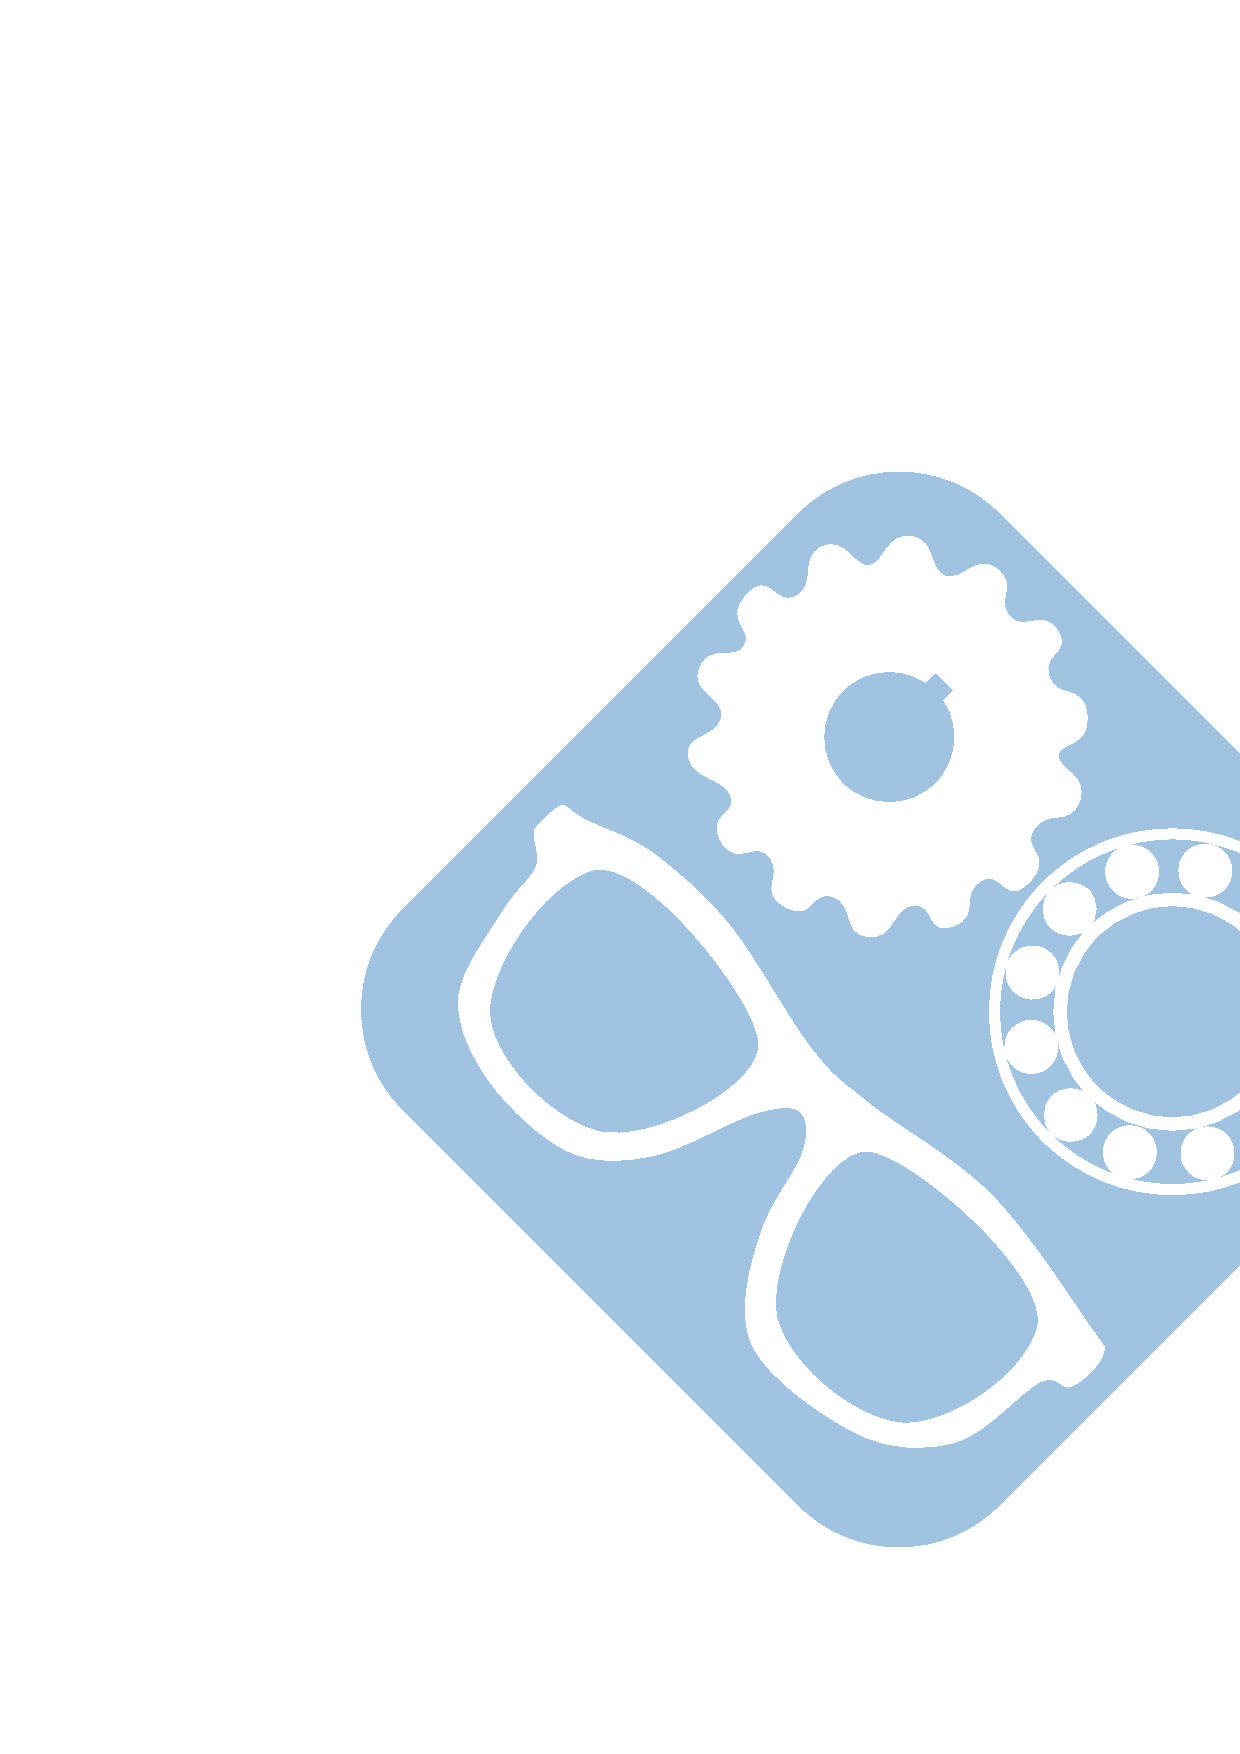
\includegraphics[width=\paperwidth,height=\paperheight,%
keepaspectratio]{../../img/fond3}%
\end{center}
\vfill
}}}

\newcommand{\BackgroundPicdeux}{%
\put(25,-30){%
\parbox[b][\paperheight]{\paperwidth}{%
\vfill
\begin{center}
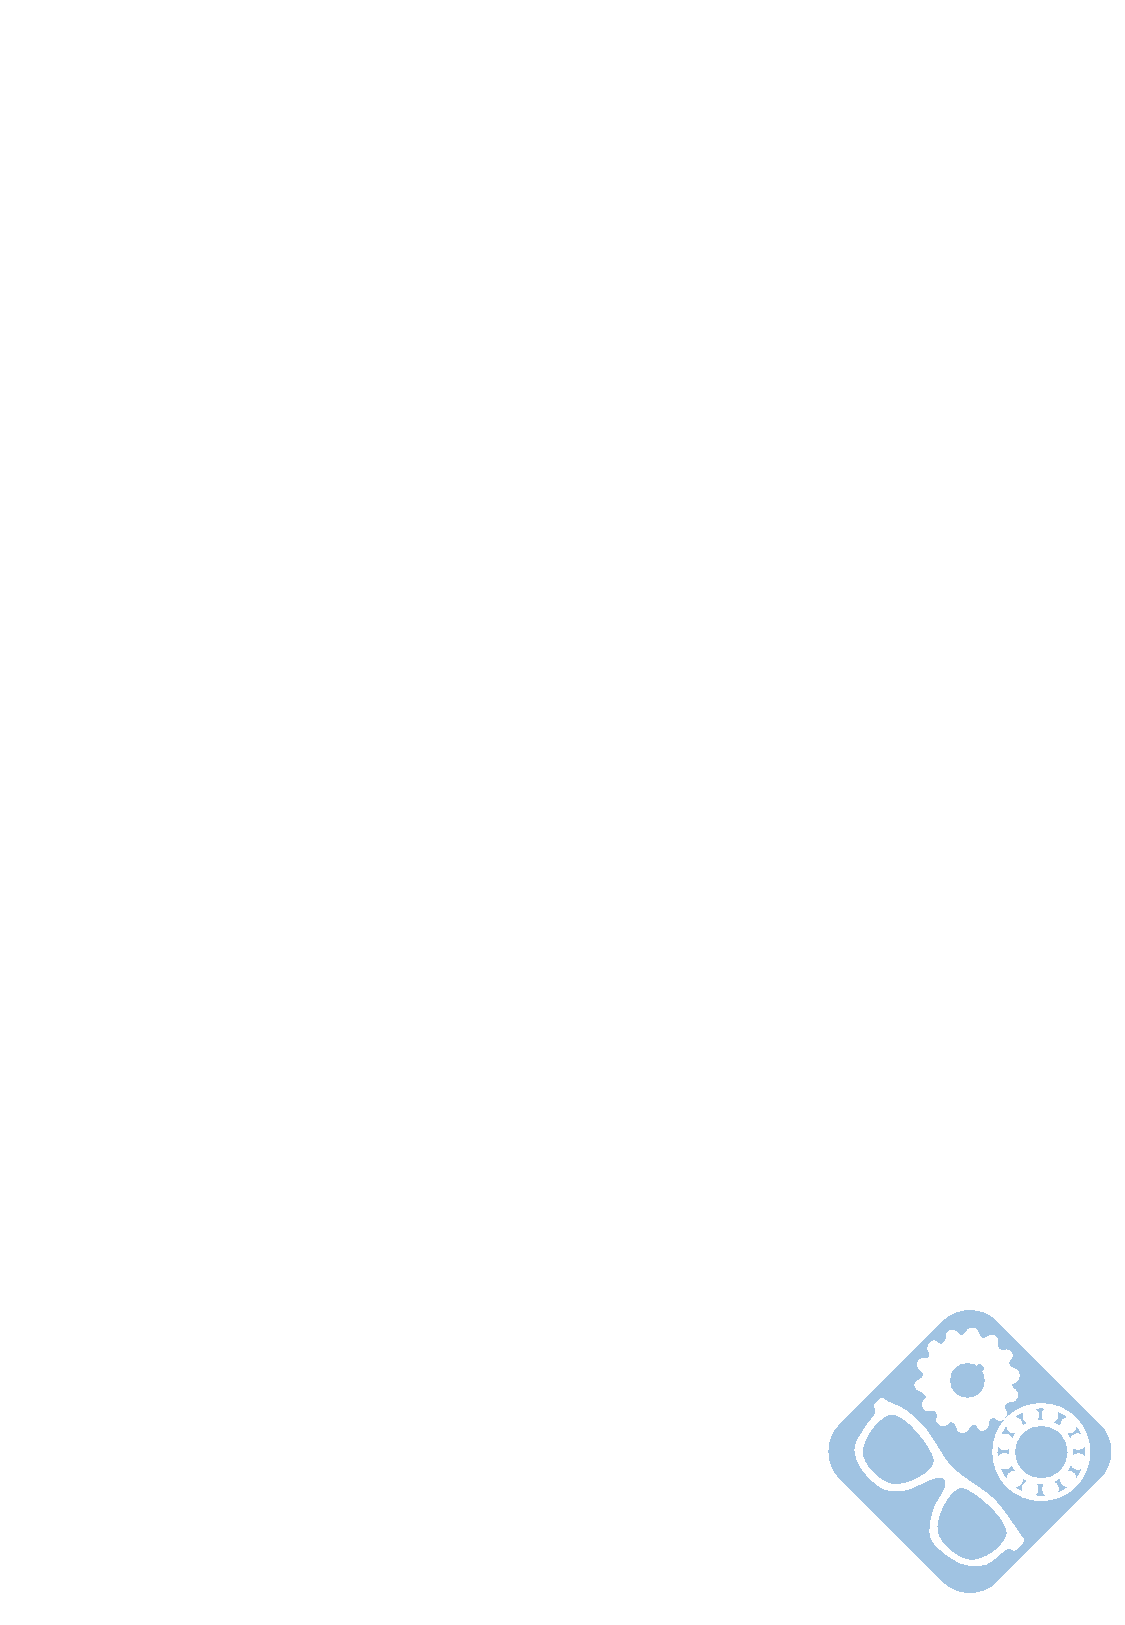
\includegraphics[width=\paperwidth,height=\paperheight,%
keepaspectratio]{../../img/fond4}%
\end{center}
\vfill
}}}

\begin{document}

\pagestyle{empty}

\vspace*{-3\baselineskip}

\AddToShipoutPicture*{\BackgroundPic}

\ifdef{\auteurdeux}{\begin{tabular}{>{\columncolor{gray!00}}m{.3\linewidth} m{.3\linewidth} >{\columncolor{gray!00}}m{.3\linewidth}}
Séquence : \sequence &  \multirow{3}{*}{\hspace{1cm}
\includegraphics[height=1.5cm]{../../img/logo}} &  \begin{flushright} \multirow{4}{*}{\hspace{1cm}\includegraphics[height=4cm]{img/qrcode}}\end{flushright}\\
Document : \type\num \\
 \institute \\
 \auteurun\\
 \auteurdeux
\end{tabular}}{\begin{tabular}{>{\columncolor{gray!00}}m{.3\linewidth} m{.3\linewidth} >{\columncolor{gray!00}}m{.3\linewidth}}
Séquence : \sequence &  \multirow{3}{*}{\hspace{1cm}
\includegraphics[height=1.5cm]{../../img/logo}} &  \begin{flushright} \multirow{4}{*}{\hspace{1cm}\includegraphics[height=4cm]{img/qrcode}}\end{flushright}\\
Document : \type\num \\
 \institute \\
 \auteurun
\end{tabular}}

\vspace{1cm}

\ifdef{\prive}{\begin{center}\colorbox{danger}{\Huge{Avec Correction}}\end{center}}{}

\begin{center}\huge{\nom}\end{center}

\vspace{2cm}

\ifdef{\imagedeux}{\begin{minipage}{0.49\linewidth}}{}
\begin{center}\includegraphics[height=5cm]{/home/renaud/Documents/Renaud/GitHub/django_education/systemes/\imageun}\end{center}
\ifdef{\imagedeux}{\end{minipage}\hfill
\begin{minipage}{0.49\linewidth}
\begin{center}\includegraphics[height=5cm]{/home/renaud/Documents/Renaud/GitHub/django_education/systemes/\imagedeux}\end{center}
\end{minipage}}{}

\vspace{5cm}


\begin{tabular}{p{.15\linewidth} >{\columncolor{white}}p{.8\linewidth}}
    \rowcolor{gray!20}
    Référence & S\sequence\ - \type\num \\
    Compétences & \competences \\
 	\rowcolor{gray!20}
    Description & \descrip \\
    Système & \systemes
  \end{tabular}

\newpage

\AddToShipoutPicture{\BackgroundPicdeux}

\pagestyle{normal}

\section{Présentation}

\subsection{La modélisation du système}

\begin{itemize}
 \item Afin de mettre en évidence l'influence des écarts géométriques et de leur contrôle, le système de la cordeuse va être utilisé et plus précisément, la partie liaison glissière.
 \item Dans un premier temps, une solution alternative afin de réaliser une liaison glissière va être utilisée. Cette solution consiste à mettre en place deux liaisons pivots glissants parallèles afin de définir une liaison glissière.
 \item Il a déjà été montré que la liaison équivalente à deux liaisons pivot-glissants est une liaison glissière. La justification par les torseurs cinématique est la suivante:
\end{itemize}

\begin{eqnarray}
& \left\{T_{1/2}\right\}=\left\{\begin{array}{c c}
0 & 0 \\
0 & 0 \\
\omega_{z12} & V_{z12,O_{1}}
\end{array}\right\}_{O_{1}}=
\left\{\begin{array}{c c}
0 & 0 \\
0 & 0 \\
\omega_{z12} & V_{z12,O_{1}}
\end{array}+\left(\begin{array}{c}
L \\
0 \\
0
\end{array}\right)\wedge
\left(
\begin{array}{c}
0 \\
0 \\
\omega_{z12}
\end{array}\right)\right\}_{O_{2}} \nonumber
\end{eqnarray}

\begin{eqnarray}
& \left\{T_{1/2}\right\}=\left\{\begin{array}{c c}
0 & 0 \\
0 & - L \times \omega_{z12} \\
\omega_{z12} & V_{z12,O_{1}}
\end{array}\right\}_{O_{2}}=
\left\{T'_{1/2}\right\}=\left\{\begin{array}{c c}
0 & 0 \\
0 & 0 \\
\omega'_{z12} & V'_{z12,O_{1}}
\end{array}\right\}_{O_{2}} \nonumber
\end{eqnarray}

\begin{itemize}
 \item Donc, $\omega_{z12}=\omega_{z12}=0$ et $V_{z12,O_{1}}=V'_{z12,O_{1}}$, ce qui montre bien que la \textbf{rotation a été supprimée} et que la translation est toujours libre. La liaison est bien une \textbf{liaison glissière}.
 \item Le choix de la conception d'une liaison glissière peut provenir de problèmes d'encombrement, de répartition des efforts,etc... Ils ne sont pas pour autant équivalents du point de vue des variations géométriques.
 \item La construction d'une liaison glissière à partir de liaisons pivot-glissant est génératrice \textbf{d'hyperstatisme} ce qui mène à des problèmes de \textbf{montabilité}.
 \item Il a déjà été vu que pour résoudre la montabilité d'un système hyperstatique, la précision de la fabrication peut être une solution.
 \item \textit{Il en existe d'autres, quelles sont-elles?}
\end{itemize}

\subsection{La modélisation des défauts}

L'objectif de ce TP va être de mettre en évidence les \textbf{défauts} qui seraient susceptibles d'empêcher le montage de la liaison. Pour cela nous allons utiliser un modèle permettant de \textbf{modéliser} l'influence de certains types de défauts: les \textbf{torseurs de petits déplacements} appliqués dans le cadre de petits écarts.

\vspace{1cm}

Ce torseur est complété de la façon suivante,:
\begin{itemize}
 \item la colonne de \textbf{gauche} modélise les déplacements en \textbf{rotation},
 \item la colonne de \textbf{droite} les déplacements en \textbf{translation}.
\end{itemize}

De plus:
\begin{itemize}
 \item une lettre \textbf{MAJUSCULE} présente un \textbf{grand} déplacement,
 \item une lettre \textbf{minuscule} présente un \textbf{petit} déplacement.
\end{itemize}

Un déplacement est défini comme grand lorsqu'il ne change pas la nature de la surface (rotation d'un cylindre autour de son axe).

Le torseur suivant en est un exemple:
\begin{eqnarray}
& \left\{T_{1/2}\right\}=\left\{\begin{array}{c c}
\alpha_{1/2} & u_{1/2,O_{1}} \\
\beta_{1/2} & v_{1/2,O_{1}} \\
\Gamma_{1/2} & W_{1/2,O_{1}}
\end{array}\right\}_{O_{1}}
\end{eqnarray}

\section{Application à l'étude}

Après cette modélisation des défauts, il est alors possible de modéliser les liaisons qui constituent la liaison glissière présentée à la figure \ref{meca_hyp}.

\begin{figure}[h!]
\begin{center}
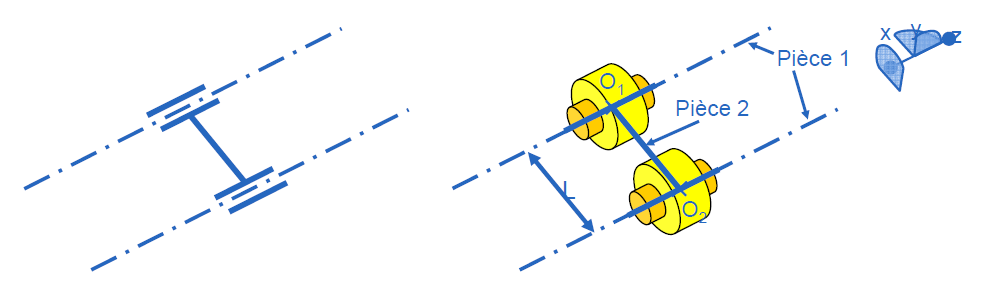
\includegraphics[width=0.8\linewidth]{img/Fig1.png}
\caption{Solution hyperstatique pour une liaison glissière}
\label{meca_hyp}
\end{center}
\end{figure}

Cette liaison est conçue en mettant en vis à vis deux paires de cylindres. On appelera:
\begin{itemize}
 \item $1a$, le cylindre appartenant à la pièce $1$ au point $O_1$,
 \item $1b$, le cylindre appartenant à la pièce $1$ au point $O_2$,
 \item $2a$, le cylindre appartenant à la pièce $2$ au point $O_1$,
 \item $2b$, le cylindre appartenant à la pièce $2$ au point $O_2$.
\end{itemize}

Ainsi, $1a$ est en contact avec $2a$ et $1b$ est en contact avec $2b$.

Il est alors possible de définir la position relative des deux pièces en écrivant deux équations:
\begin{eqnarray}
& & \left\{T_{1/2}\right\}=\left\{T_{1/1a}\right\}+ \left\{T_{1a/2a}\right\}+\left\{T_{2a/2}\right\} \nonumber \\
& & \left\{T'_{1/2}\right\}=\left\{T_{1/1b}\right\}+ \left\{T_{1b/2b}\right\}+\left\{T_{2b/2}\right\}, avec \nonumber \\
& & \left\{T_{1/2}\right\}+\left\{T'_{2/1}\right\}=\left\{0\right\}
\end{eqnarray}

Les torseurs $\left\{T_{1/1a}\right\}$, $\left\{T_{2a/2}\right\}$, $\left\{T_{1/1b}\right\}$ et $\left\{T_{2b/2}\right\}$ correspondent aux défauts géométriques des surfaces par rapport à la pièce.

Les torseurs $\left\{T_{1a/2a}\right\}$ et $\left\{T_{1b/2b}\right\}$ correspondent aux jeux entre les pièces dans les liaisons en $O_1$ et $O_2$.

\section{Les écarts géométriques}

Afin de mettre en évidence l'influence des écarts géométriques et de leur contrôle, le système de la cordeuse va être utilisé et plus précisément, la partie liaison glissière.

\subsection{La modélisation des défauts}

\paragraph{Question 1:} Quels sont les grands déplacements qui ne modifie pas cette surface ?

\reponse[2]

\paragraph{Question 2:} Qu'en déduire quant à la nature de la surface ?

\reponse[2]

\paragraph{Question 3:} Écrire les torseurs des écarts concernant les surfaces en $O_1$ et en $O_2$ de la pièce 1 puis de la pièce 2.

\begin{minipage}{0.48\linewidth}
\begin{eqnarray}
& \left\{T_{1/1a}\right\}=\left\{\begin{array}{m{2cm} c}
 &  \\
 &  \\
 & 
\end{array}\right\}_{O_{1}}
\end{eqnarray}
\end{minipage}
\hfill
\begin{minipage}{0.48\linewidth}
\begin{eqnarray}
& \left\{T_{2a/2}\right\}=\left\{\begin{array}{m{2cm} c}
 &  \\
 &  \\
 & 
\end{array}\right\}_{O_{1}}
\end{eqnarray}
\end{minipage}

\begin{minipage}{0.48\linewidth}
\begin{eqnarray}
& \left\{T_{1/1b}\right\}=\left\{\begin{array}{m{2cm} c}
 &  \\
 &  \\
 & 
\end{array}\right\}_{O_{2}}
\end{eqnarray}
\end{minipage}
\hfill
\begin{minipage}{0.48\linewidth}
\begin{eqnarray}
& \left\{T_{2b/2}\right\}=\left\{\begin{array}{m{2cm} c}
 &  \\
 &  \\
 & 
\end{array}\right\}_{O_{2}}
\end{eqnarray}
\end{minipage}

Pour le moments, le jeu entre les surfaces des deux pièces sera considéré comme nul, ainsi $\left\{T_{1a/2a}\right\}=\left\{0\right\}$ et $\left\{T_{1b/2b}\right\}=\left\{0\right\}$

\paragraph{Question 4:} Calculer les torseurs $\left\{T_{1/2}\right\}_{O_1}$ et $\left\{T'_{1/2}\right\}_{O_2}$. Les déplacer au même point ($O_2$) et écrire les équations scalaires liées au système suivant: $\left\{T_{1/2}\right\}+\left\{T'_{2/1}\right\}=\left\{0\right\}$.

\newpage

\paragraph{Question 5:} Lister les \textbf{grands} déplacements qui s'écrivent en fonction de \textbf{grands} déplacements.

\reponse[4]

\paragraph{Question 6:} Ceux-ci sont normalement toujours des degrés de liberté dans la liaison équivalente, est-ce vrai ?

\reponse[2]

\paragraph{Question 7:} Lister les \textbf{grands} déplacements qui ne s'écrivent qu'en fonction de \textbf{petits} déplacements.

\reponse[4]

Ceux-ci sont normalement bloqués par la liaison équivalente.

\paragraph{Question 8:} Lister les \textbf{petits} déplacements qui ne s'écrivent qu'en fonction de \textbf{petits} déplacements.

\reponse[4]

Ces équations génèrent des contraintes géométriques. Afin de pouvoir spécifier les défauts, essayer de regrouper les variables par pièce. Par exemple, au lieu d'écrire: $x_{1/1a}+x_{1b/1}$, écrire plutôt $x_{1b/1a}$.

\paragraph{Question 9:} Quels sont les défauts qui apparaissent sur vos équations. Est-ce logique ?

\reponse[2]

Normalement, les défauts qui devraient alors apparaître sont ceux représentés sur la figure \ref{degres_hyp}.

\begin{figure}[h!]
\begin{center}
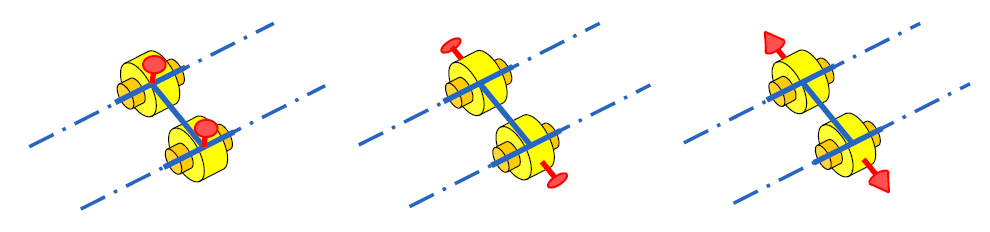
\includegraphics[width=0.8\linewidth]{img/Fig2.png}
\caption{Degrés d'hyperstatisme de la solution}
\label{degres_hyp}
\end{center}
\end{figure}

\paragraph{Question 10:} Vos résultats sont-ils compatibles avec ceux présentés sur la figure \ref{degres_hyp} ?

\reponse[2]

\subsection{Conclusion}

Nous avons vu dans cet exemple que des degrés d'hyperstatisme dans un système généraient des contraintes à prendre en compte concernant les défauts géométriques.

Nous savons que la solution qui a été choisie dans le cadre de la cordeuse consiste à rendre le système isostatique, ce qui a pour effet de faire disparaître ces problèmes.

Nous aurions pu tout aussi bien ajouter du jeu dans la conception afin de garantir la montabilité. Ceci aurait eu pour effet mathématiquement de rendre non nuls les torseurs $\left\{T_{1a/2a}\right\}$ et $\left\{T_{1b/2b}\right\}$

\newpage

\section{Les jeux}

\begin{minipage}{0.48\linewidth}
Dans cette partie, nous allons étudier l'influence des jeux dans la montabilité des systèmes.

Nous allons pour cela utiliser les montages de roulements à rouleaux disponibles dans le labo de sciences industrielles.

Ceux-ci sont constitués de deux liaisons en parallèle entre un arbre \textbf{1} et un alésage \textbf{2}.
\end{minipage}
\hfill
\begin{minipage}{0.45\linewidth}
 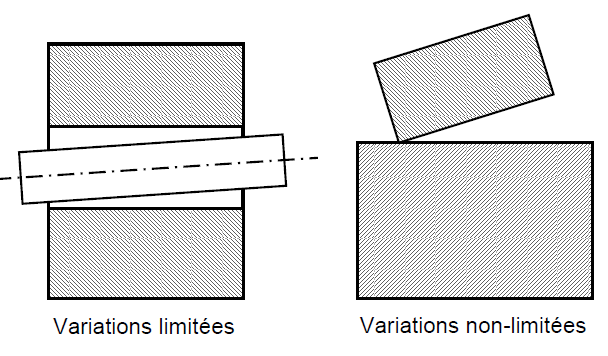
\includegraphics[width=0.8\linewidth]{img/Fig3.png}
\end{minipage}

\subsection{Modélisation des défauts et des jeux}

\paragraph{Question 11:} Modéliser cinématiquement cet assemblage et le paramétrer (Points, liaisons, repères). Afin de simplifier l'étude, la bague extérieure du roulement sera liée à l'alésage et la bague intérieure sera liée à l'arbre.

Définir les surfaces de contact.

\paragraph{Question 12:} Modéliser les torseurs d'\textbf{écarts} de ces surfaces ainsi que les torseurs de \textbf{jeu}.

\reponse[8]

\paragraph{Question 13:} Définir les torseurs des positions relatives des pièces et résoudre le système qui lie ces torseurs.

\reponse[8]

\subsection{Comment les jeux compensent les défauts}

\paragraph{Question 14:} Déterminer quelles composantes des torseurs de jeu doivent être non-nulles afin de compenser les défauts géométriques des pièces.

\reponse[4]

\paragraph{Question 15:} Cette conclusion vous paraît-elle logique et correspond-t-elle à la réalité?

\reponse[2]

\subsection{Conclusion}

Ce TP a donc permis dans un premier temps de déterminer les défauts géométriques des pièces ainsi que leur influence. Il a ensuite permis de montrer que les jeux permettaient de compenser ces problèmes.

Cependant, les jeux peuvent générer des problèmes de leur côté (vibrations, ...) il ne faut donc pas en abuser, c'est pour cela que les défauts géométriques ainsi que les jeux devront être limités, c'est ce que nous feront plus tard dans le cours de spécifications.


\end{document}
